\documentclass[border=10pt]{standalone}
\usepackage[svgnames]{xcolor}
\usepackage{amsmath}
\usepackage{pgfplots}
\pgfplotsset{compat=newest}
\usepackage[sfdefault]{FiraSans}
\usepackage{FiraMono}
\renewcommand*\familydefault{\sfdefault}
\begin{document}
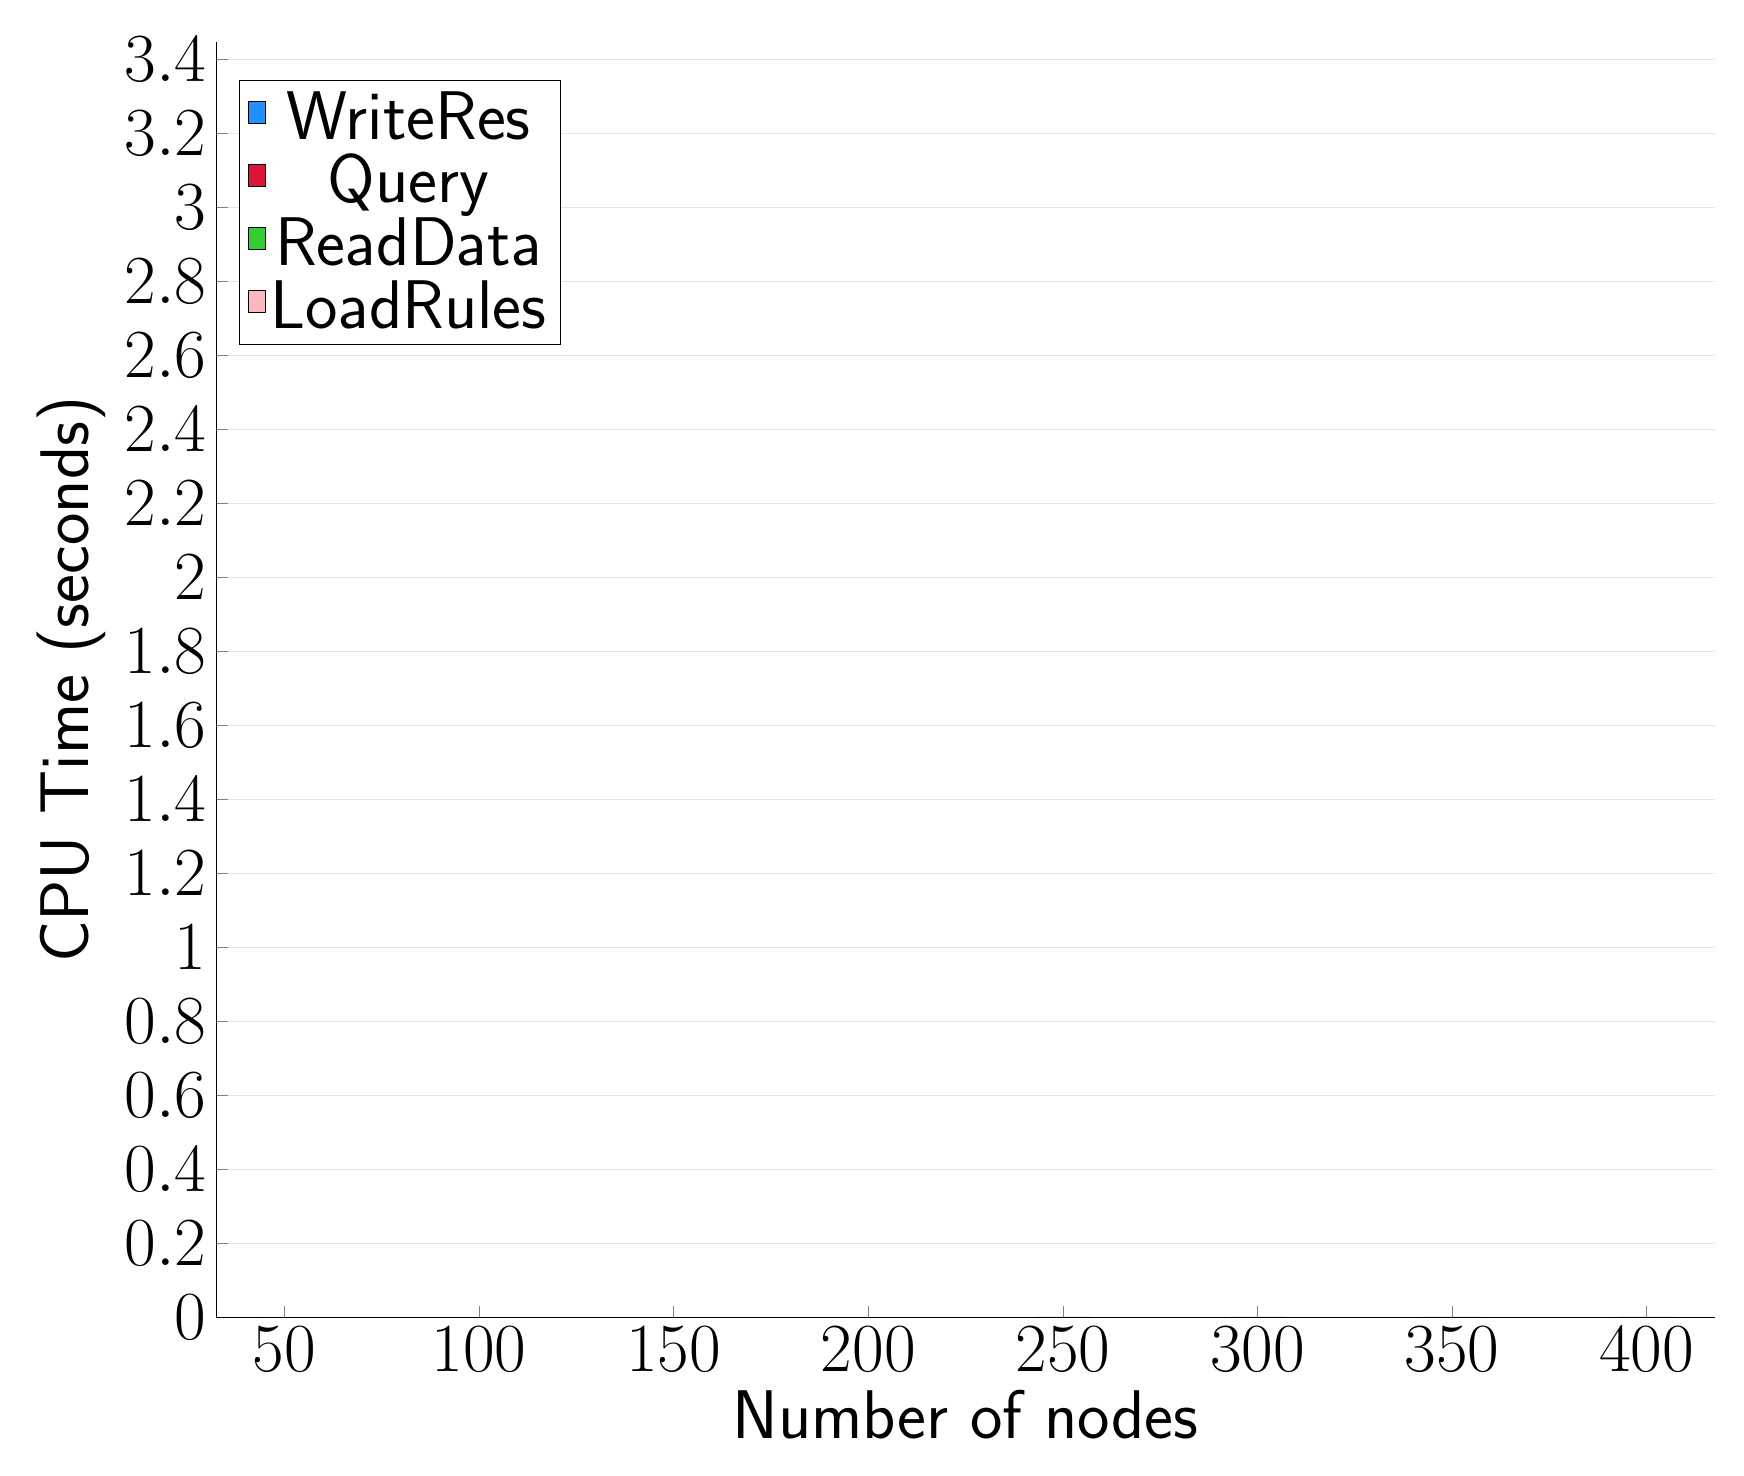
\begin{tikzpicture}
\begin{axis}[
   ybar stacked,
   width=1.7\textwidth,
   bar width=0.7cm,
   ymajorgrids, tick align=inside,
   major grid style={draw=gray!20},
   xtick=data,
   ymin=0, ymax=3.4459999999999997,
   axis x line*=bottom,
   axis y line*=left,
   enlarge x limits=0.05,
   legend style={
       at={(0.23, 0.97)},
       anchor=north east,
       legend columns=1,
       font=\Huge,
   },
   ylabel={CPU Time (seconds)},
   xlabel={Number of nodes},
   label style={font=\Huge},
   tick label style={font=\Huge},
]
\addlegendimage{fill=DodgerBlue, draw=black, line width=0.2pt}
\addlegendentry{WriteRes}
\addlegendimage{fill=Crimson, draw=black, line width=0.2pt}
\addlegendentry{Query}
\addlegendimage{fill=LimeGreen, draw=black, line width=0.2pt}
\addlegendentry{ReadData}
\addlegendimage{fill=LightPink, draw=black, line width=0.2pt}
\addlegendentry{LoadRules}
\addplot +[fill=LightPink, draw=black, line width=0.2pt] coordinates {
(50, 0.0006014999999999996)
(100, 0.0006193000000000003)
(150, 0.0006062999999999997)
(200, 0.0006058999999999998)
(250, 0.000603)
(300, 0.0006015999999999997)
(350, 0.0006107000000000003)
(400, 0.0006056999999999998)
};
\addplot +[fill=LimeGreen, draw=black, line width=0.2pt] coordinates {
(50, 0.0001741000000000005)
(100, 0.00021639999999999978)
(150, 0.00025129999999999993)
(200, 0.0002952)
(250, 0.0003327)
(300, 0.00037579999999999965)
(350, 0.00041819999999999976)
(400, 0.00046269999999999975)
};
\addplot +[fill=Crimson, draw=black, line width=0.2pt] coordinates {
(50, 1.5399999999999958e-05)
(100, 2.2500000000000113e-05)
(150, 2.5700000000000045e-05)
(200, 3.0700000000000184e-05)
(250, 3.609999999999967e-05)
(300, 4.2000000000000384e-05)
(350, 4.7000000000000356e-05)
(400, 5.440000000000014e-05)
};
\addplot +[fill=DodgerBlue, draw=black, line width=0.2pt] coordinates {
(50, 0.00011339999999999996)
(100, 0.00015809999999999997)
(150, 0.00020679999999999988)
(200, 0.00024959999999999967)
(250, 0.0002949000000000005)
(300, 0.0003434999999999998)
(350, 0.0003884999999999995)
(400, 0.00043140000000000046)
};
\end{axis}
\end{tikzpicture}

\end{document}
